\pagestyle{MyStyle}

\chapter[Introduction]{Introduction}
\label{ch:intro}

\vspace{3cm}

\begin{refsection}
\newpage
\section*{The brain connectome}
The brain is a supremely complex organ in the human body. The adult human brain consists of approximately 100 billion neurons and 150 trillion synapses \citep{HerculanoHouzel2012TheRY}. Through axonal projections and synapses, neurons are wired into neural circuits that interconnect to one another to form the large-scale brain network, namely the connectome \citep{sporns_human_2011}. Mapping the microscale connectome of the human brain is extremely challenging due to the huge amount of synapses and the extremely densely packed neuronal circuits, with the largest reconstruction of ~500,000 cubic micrometers of the mouse connectome available at present \citep{Motta2019DenseCR}. To achieve an overall view of the whole-brain connectome, the macroscale human brain connectome formed by brain regions and interregional brain connectivity has been reconstructed taking advantage of non-invasive brain imaging techniques such as magnetic resonance imaging (MRI) \citep{Bullmore2009ComplexBN,sporns_human_2011}. The macroscale brain connectivity usually describes anatomical white matter tracts that are reconstructed using diffusion weighted imaging (DWI) \citep{Hagmann2007MappingHW} or the temporal relationship of intrinsic neural activities measured by functional MRI (fMRI) \citep{Friston1994FunctionalAE}. The macroscale brain connectome has been claimed as an efficient network that enables both functional specialization and functional integration within the whole brain \citep{bullmore_economy_2012}. It supports a rich body of functional dynamics and interactions that underlie human cognition and behaviors, evidenced by associations between the connectome organization and cognitive processing in humans \citep{Heuvel2009EfficiencyOF, Baggio2015RichCO,barbey2018network} and brain dysconnectivity in mental disorders \citep{crossley2014hubs,Fornito2015ReconcilingAO}. Therefore, the macroscale brain connectome provides an invaluable model for understanding the neural basis of human cognition and the neuropathology of brain disorders.

\section*{Aim of this thesis}
One of the major challenges in the field of the connectomics is to understand the wiring principle of the human brain connectome. What shapes brain connectivity and the connectome architecture in the human brain? This thesis aims to address this question by integrating multiscale data, namely, data from different levels of nervous system organization, including brain transcriptomics, histology, and multi-modal MRI. Furthermore, this thesis aims to examine multiscale, multimodal connectome abnormalities in psychiatric disorders, in particular schizophrenia, to provide insights into the neuropathology of the disorder. We expect our integrative approaches to be useful in gaining a better knowledge of the wiring principle of the human brain connectome, and ultimately, to gain a deeper understanding of human cognition, behavior and brain disorders.

\section*{General background}
\subsection*{Topological characteristics of the connectome}
The macroscale brain connectome is a complex network composed of comprehensive sets of connections between brain areas. Mathematically, a network, or a graph, is defined as a set of nodes and edges. Concerning the human brain network, nodes are usually defined according to the parcellation of unique brain regions, which are established based on cortical cytoarchitecture \citep{brodmann1909vergleichende}, gyrification \citep{DESIKAN2006968}, connectivity profiles \citep{Fan2016TheHB}, or a combination of multiple modalities \citep{Glasser2016AMP}. Edges are defined as inter-areal structural and functional connectivity among brain regions. Structural connectivity in the human brain commonly reflects white matter bundles reconstructed using DWI \citep{Hagmann2008MappingTS}. The size of white matter bundles or the microscopic features such as myelination can be inferred and taken as the weight of structural connectivity. Functional connectivity in the human brain is characterized as the statistical dependency of brain activity between brain regions \citep{Friston2011FunctionalAE}, such as the synchrony of blood oxygenation level-dependent (BOLD) signals derived from resting-state fMRI. Recent studies on the human structural and functional connectome have revealed the most fundamental attribute of the connectome: the capability of promoting segregation and integration of neural information \citep{Sporns2013NetworkAF}.

Neural information segregation complies with the long-standing argument of brain functional specialization, with evidence from a wide range of anatomical, physiological, and neuroimaging studies showing different brain areas to be specialized for different cognitive domains \citep{Finger1994OriginsON}. Connectome analyses add to this by demonstrating the architecture of communities in the functional connectome \citep{Sporns2016ModularBN}. Brain regions within a community are way more densely connected to each other in contrast to being connected to nodes outside the community. The observed sets of communities coincide with the distributed “resting-state networks” (RSNs) that are derived by independent component analysis (ICA) on whole-brain resting-state fMRI data \citep{Beckmann2005InvestigationsIR}. The RSNs correspond to functional systems in distinct behavioral or cognitive domains \citep{smith2009correspondence,Laird2011BehavioralIO}, including the default-mode (DMN), frontoparietal control, dorsal-attention, ventral-attention, sensorimotor, and visual networks \citep{Power2011FunctionalNO,thomas2011organization}. These spatially-distributed functional systems have been found to be supported by underlying anatomical connections \citep{Heuvel2009FunctionallyLR} and to be globally integrated via pivotal “hub” regions to facilitates complex brain functions \citep{van_den_heuvel_network_2013}.

Neural information integration describes the integration of neural information among distributed functional systems and is served by a specific set of brain hub regions \citep{Heuvel2013AnAS}. Hub regions are mostly located in multimodal association areas, such as the precuneus, insular cortex, superior frontal cortex, temporal cortex, and lateral parietal cortex \citep{van_den_heuvel_network_2013}. Furthermore, these hub regions are not only highly connected to the rest of the brain, but also tightly connected with each other, forming a “rich club”  \citep{vanDenHeuvel2011RichclubOO,Griffa2018RichclubNF}. Rich-club areas and their connections enable short communication pathways among non-rich-club, peripheral areas, thus promote network efficiency with a trade-off against high wiring cost of connections among distant hub regions \citep{vanDenHeuvel2012HighcostHB}. These central regions are also flexible over time, indicative of the capability of dynamically switching brain states from more localized processing (i.e., segregation) to more globalized synchronization (i.e., integration) \citep{Zalesky2014TimeresolvedRB,Shine2015TheDO}. Such a flexibility enables the brain to adapt to changing demands \citep{Cole2013MultitaskCR} and facilitates faster and more accurate cognitive performance \citep{Shine2015TheDO}. 

Together, neural information segregation and integration are two fundamental features of the human brain connectome. These two features play a key role in complex brain dynamics underlying human's cognition and behavior. One major goal of the current thesis is to understand the origin and emergence of these important topological features of the human brain connectome.

\subsection*{Neurobiological basis of the connectome}
The above-mentioned features of the human human connectome are mostly discussed in the context of a computational perspective, leaving the question of the connectome's underlying biological basis open. In recent years, studies have bridged the microscale cellular and molecular brain structure to the macroscale connectome organization to uncover the neurobiological mechanisms of the connectome \citep{Scholtens2018MultimodalCI,Heuvel2019MultiscaleNO}. Brain regions are known to show a large variety of cellular composition \citep{brodmann1909vergleichende,von1925cytoarchitektonik}, for example, larger and more spinous pyramidal cells are observed in associative prefrontal cortex compared to primary visual cortex \citep{elston2001pyramidal,elston2003cortex}. Extending this cytoarchitectonic variation, studies have further proposed that the inter-regional cytoarchitectonic differentiation plays a critical role in shaping cortico-cortical connections \citep{barbas2015general}. Brain regions with similar cytoarchitecture are more likely to be connected both anatomically and functionally \citep{barbas2015general,beul2015predictive,beul2017predictive,goulas2017principles}. Moreover, cortical cytoarchitecture is also associated with functional segregation and integration in the brain. Paralimbic regions with an undifferentiated laminar structure, along with absent or disrupted cortical layer IV, are prominently involved in between-network connectivity across functional networks \citep{Wylie2015BetweennetworkCO}. Densely connected rich-club regions show the largest basal dendritic tree size, spine density, and neuron soma size of layer III pyramidal neurons \citep{scholtens2014linking,Heuvel2015BridgingCA,VANDENHEUVEL2016293}. These observations suggest a highly complex neuronal structure in rich-club regions, such that rich-club regions can deal with the costly neural information integration. 

Extending the association between the macroscale connectome and microscale brain cytoarchitecture, the connectome organization has been claimed to be related to the underlying genetic information. By combining gene expression and brain connectivity in the rodent brain, it has been shown that the existence of anatomical connectivity could be predicted by gene expression levels \citep{Wolf2011GeneEI}, and anatomically-connected regions tended to show more similar expression profiles \citep{French2011RelationshipsBG}. Genes that are mostly correlated with anatomical connectivity are enriched for gene sets involved in neuronal development and axon guidance \citep{French2011RelationshipsBG}. Moreover, the topology of macroscale functional networks in the human brain is related to the co-expression of genes that are enriched for ion channels \citep{richiardi2015correlated} and genes that are preferentially expressed in human supragranular cortical layers \citep{krienen2016transcriptional}. Rich-club regions also show a differentiated level of gene expression coupling for genes regulating the oxidative synthesis and metabolism of ATP, which provide the energetic substrate for neuronal communication \citep{Fulcher2016ATS}. These findings suggest a cross-scale association of the microscale transcriptomics and cytoarchitecture, and the macroscale connectome organization.

\begin{figure}[h]
    \centering
    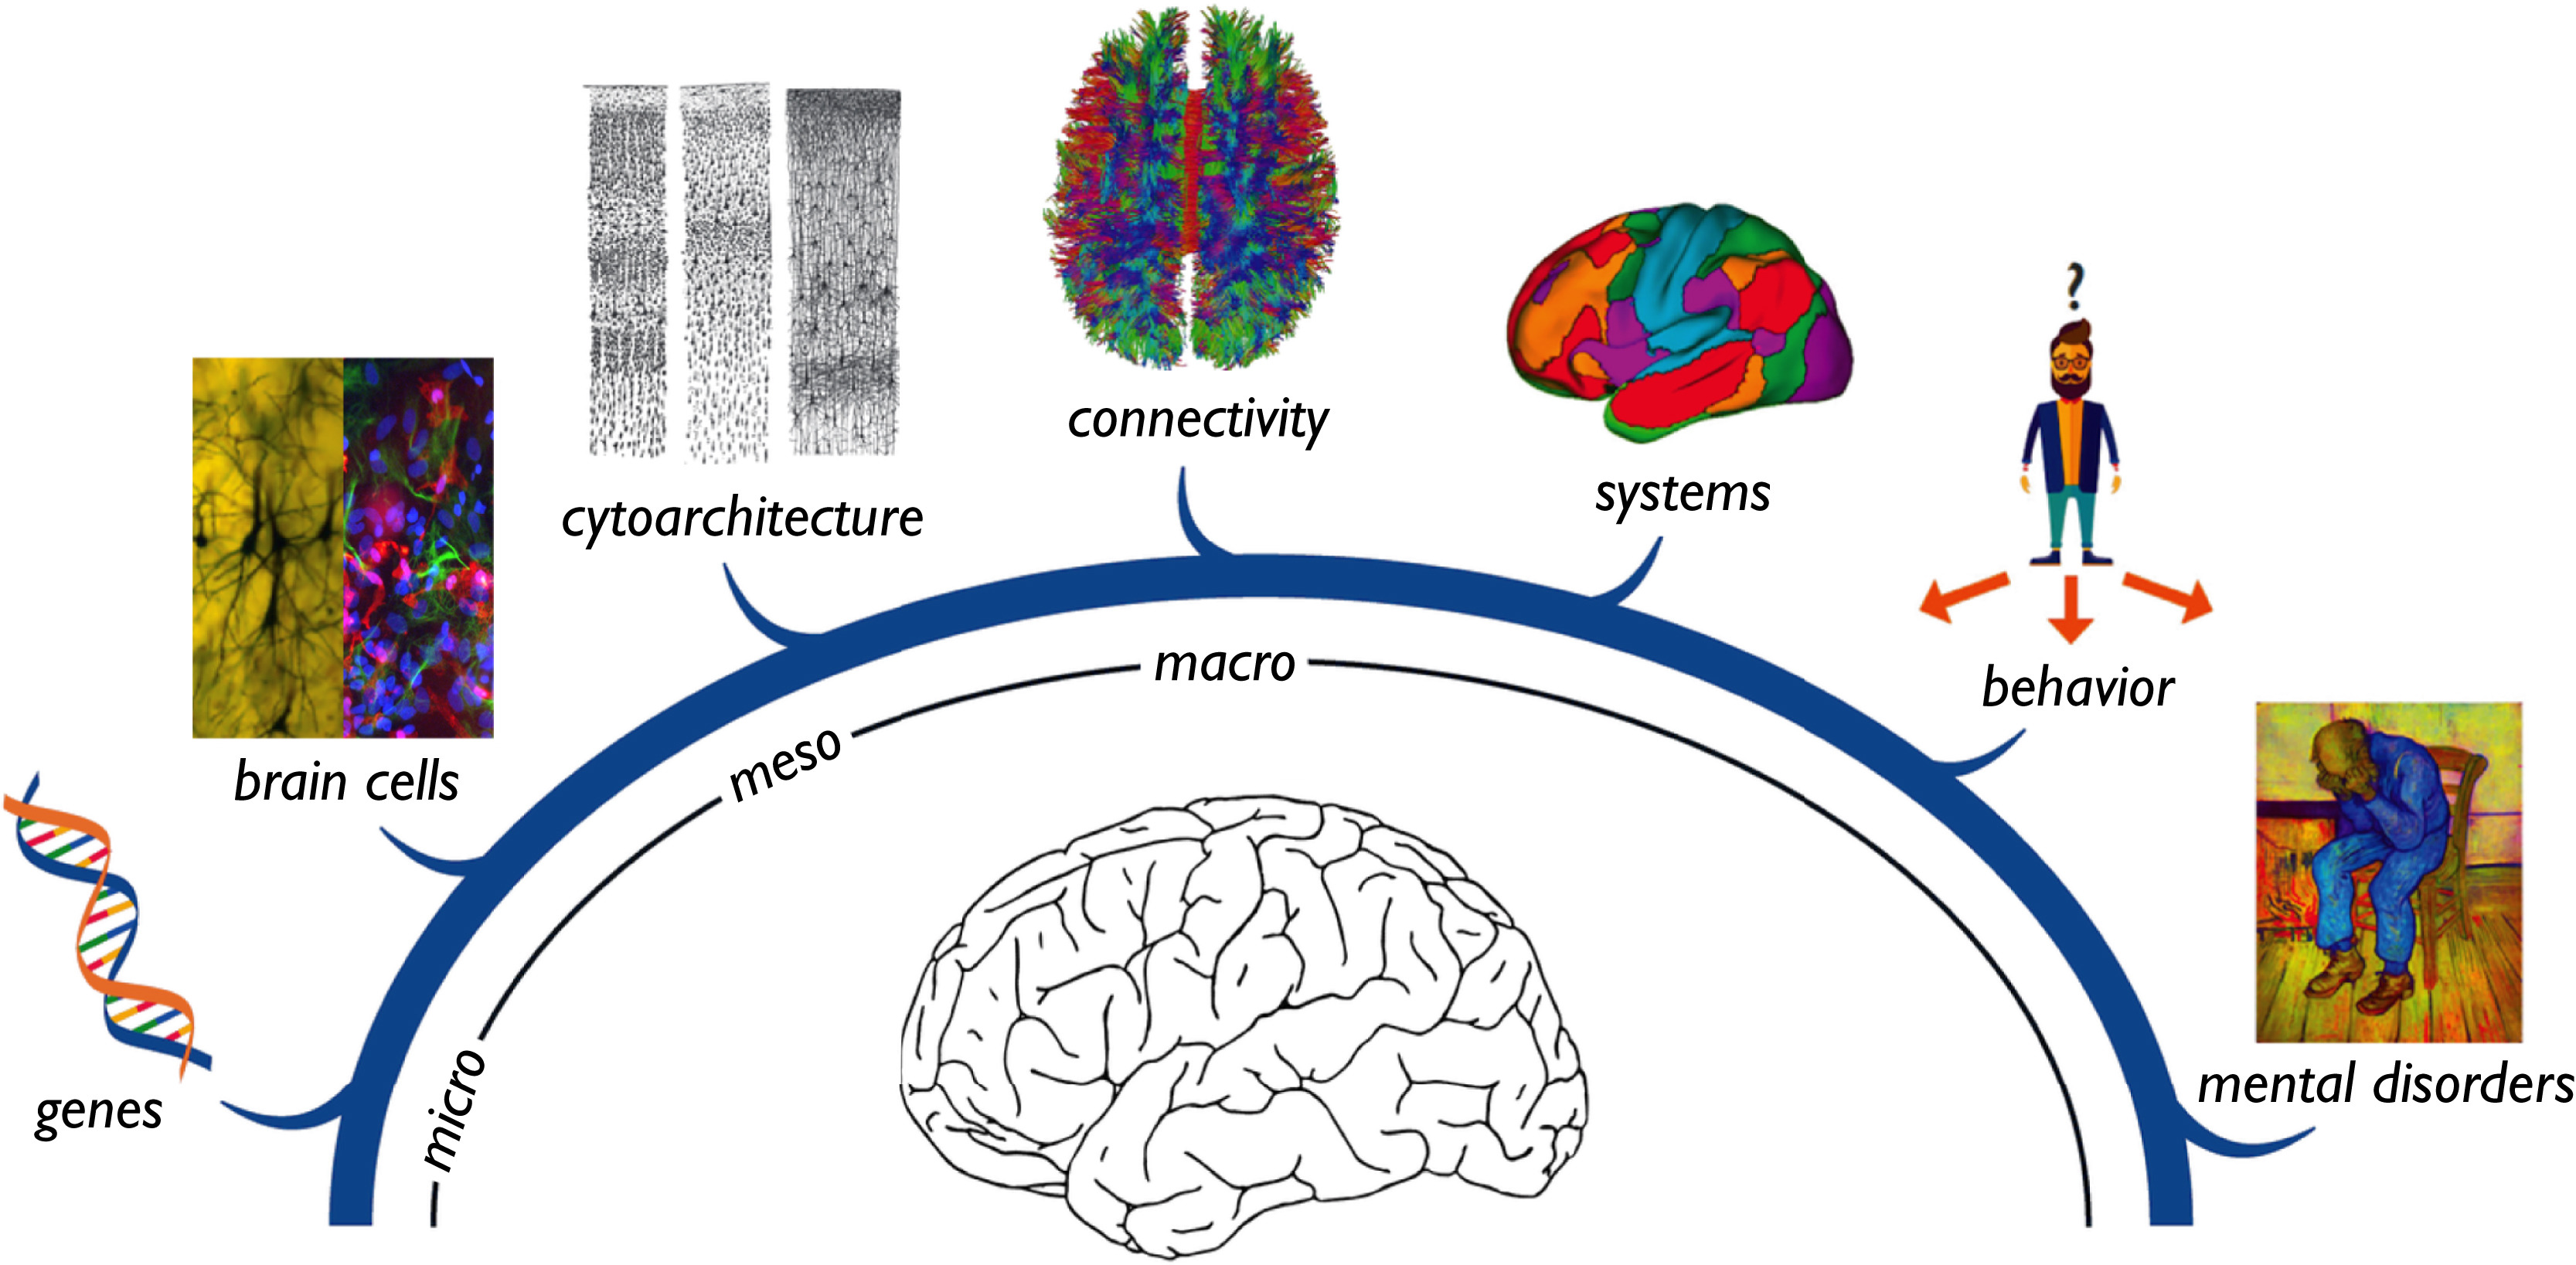
\includegraphics[width=\linewidth]{images/introFig1.jpg}
    \caption{An overview of multiscale neuroscience. The microscale, mesoscale, and macroscale human brain structure and function are integrated for an understanding of human behavior and mental disorders. Selected examples from left to right describe genes, brain cells, cytoarchitecture, connectivity, functional systems, behavior and mental disorders. Reprinted from “Multiscale Neuroscience of Psychiatric Disorders”, by Authors M.P. van den Heuvel et al., 2019, Biological Psychiatry, 86(7), 512-522. Copyright [2019] by the Society of Biological Psychiatry. Reprinted with permission.}
    \label{introFig1}
\end{figure}


\subsection*{Multiscale neuroscience and schizophrenia}
The association across different scales of brain organization can be noted not only in the healthy brain, but also in brains of patients with psychiatric disorders (Figure \ref{introFig1}). Schizophrenia is a psychiatric disorder characterized by hallucinations, delusions, a loss of initiative, cognitive dysfunction, as well as disruptions of brain connectivity \citep{Stephan2009DysconnectionIS}. Since around 100 years ago, pioneering psychiatrists Carl Wernicke (1848-1905) and Eugen Bleuler (1857-1939) hypothesized a loosening of association fibers in the brain of schizophrenia. Empirical MRI studies have provided further evidence for the widespread disruptions of interregional brain connectivity in schizophrenia \citep{EllisonWright2009MetaanalysisOD,Klauser2017WhiteMD,Fitzsimmons2013ReviewOF}, in particular disrupted connectivity between hub/rich-club regions of the brain \citep{vanDenHeuvel2013AbnormalRC,Klauser2017WhiteMD}. These alterations of hub/rich-club connectivity parallel with decreased brain network efficiency \citep{Zalesky2011DisruptedAF}, suggesting the disrupted neural information integration in schizophrenia.

A rich body of brain cytoarchitectonic studies has further shown alterations of microscale neuronal projections in schizophrenia \citep{Bakhshi2015TheNO}. For example, dendritic spines pathology has been observed in schizophrenia, in particular for layer III pyramidal neurons in prefrontal cortex, indicating disruptions of cortico-cortical and cortico-thalamus excitatory connections in schizophrenia \citep{Glausier2013DendriticSP}. Furthermore, a cross-scale study has revealed that brain regions with a more decreased spine density of pyramidal neurons showed more connectivity disruptions at the macroscale \citep{VANDENHEUVEL2016293}, confirming the macro-micro linkage in the neuropathology of schizophrenia. 

The micro-macro relationship in schizophrenia is further reflected by the underlying genetic signatures. Genome-wide association studies (GWAS) have shown that schizophrenia is a highly polygenic disorder \citep{Ripke2014BiologicalIF}, namely, a disorder led by multiple genes with additive small effects. The recent GWAS on 40,675 schizophrenia patients and 64,643 controls have identified >100 genomic risk loci and >300 risk genes \citep{Pardias2018CommonSA}. The identified genes have been shown to be associated with the formation of microscopic neuronal projection \citep{Pardias2018CommonSA}. More intriguingly, genetic variants related to risks in schizophrenia have been found to be enriched in interneuron-linked genes and can be predictive of functional activity of parvalbumin-biased brain regions \citep{Anderson2018TheTL}. Schizophrenia polygenic risk scores have shown to negatively correlate with macroscale functional connectivity in the visual network, default-mode network, and frontoparietal network \citep{Cao2020FunctionalCA}. Cortical transcriptions of schizophrenia-risk genes have also been noted to be associated with the macroscale disconnectivity pattern in schizophrenia, showing that brain regions with higher gene expression were more disconnected at the macroscale \citep{Romme2017ConnectomeDA}. 

Taken together, the genetic variants to the risk of schizophrenia, the differentiated gene expression of schizophrenia risk genes, the cellular pathological abnormalities, and the macroscale connectome alterations in schizophrenia may interactively influence each other rather than being independent. Integrating multiscale neuroscience data of schizophrenia enable us to gain a better understanding of the complex etiology of the disease.


\section*{Outline of the thesis}
This thesis aims to explore the neurobiological mechanisms underlying the human brain connectome and to scrutinize the multiscale neuropathology of schizophrenia. To do so, the following six chapters are included in this thesis. In \textbf{Chapter 2}, I use the state-of-the-art BigBrain histological dataset \citep{amunts2013bigbrain} and examine how cortical laminar cytoarchitecture relates to the organization of the macroscale brain connectome. In \textbf{Chapter 3}, I delve into the organizing principles of functional networks from the perspective of evolutionary genetics. I examine the expansion of cognitive functional networks in human evolution, and I investigate gene expression levels of human-accelerated genes (HAR genes) in those human-expanded cognitive functional networks. In addition, I demonstrate associations between human-accelerated genes and cognitive abilities and risks of psychiatric disorders in today's population based on recent GWAS results. \textbf{Chapter 4} further introduces a web-application, GAMBA, which can be used for annotating transcription-neuroimaging associations among a wide range of neuroimaging phenotypes of the healthy and diseased brain. In \textbf{Chapter 5}, I focus on schizophrenia and examine alterations of rich-club organization of the macroscale brain connectome and structural-functional connectivity coupling in first-episode, medication-naïve schizophrenia patients. In \textbf{Chapter 6}, I use magnetization transfer (MT) imaging data to provide an estimation of the microscale neuropathology in schizophrenia, and examine how microscale neuropathology correlate to macroscale dysconnectivity in schizophrenia. Finally, \textbf{Chapter 7} summarizes the findings in this thesis and discusses methodological considerations and future directions.

\printbibliography[heading=subbibliography]

\end{refsection}